\documentclass[a0paper,portrait]{xebaposter}
%%%%%%%%%%%%%%%%%%%%%%%%%%%%%%%%%%%%%%%%%%%%%%%%
% Language, Encoding and Fonts
% http://en.wikibooks.org/wiki/LaTeX/Internationalization
%%%%%%%%%%%%%%%%%%%%%%%%%%%%%%%%%%%%%%%%%%%%%%%%
% Select encoding of your inputs. Depends on
% your operating system and its default input
% encoding. Typically, you should use
%   Linux  : utf8 (most modern Linux distributions)
%            latin1 
%   Windows: ansinew
%            latin1 (works in most cases)
%   Mac    : applemac
% Notice that you can manually change the input
% encoding of your files by selecting "save as"
% an select the desired input encoding. 
\usepackage[utf8]{inputenc}
% Make latex understand and use the typographic
% rules of the language used in the document.
\usepackage[english]{babel}
% Use the vector font Latin Modern which is going
% to be the default font in latex in the future.
%\usepackage{helvet}
% Change the default font family from roman to sans serif
\renewcommand{\familydefault}{\sfdefault} % for text
%\usepackage[helvet]{sfmath} % for math
% Choose the font encoding
\usepackage[T1]{fontenc}

\usetikzlibrary{arrows}

\definecolor{zzttff}{rgb}{0.6,0.2,1}
\definecolor{zzttqq}{rgb}{0.6,0.2,0}
\definecolor{qqqqff}{rgb}{0,0,1}
\definecolor{qqwuqq}{rgb}{0,0.4,0}

%%%%%%%%%%%%%%%%%%%%%%%%%%%%%%%%%%%%%%%%%%%%%%%%
% Graphics and Tables
% http://en.wikibooks.org/wiki/LaTeX/Importing_Graphics
% http://en.wikibooks.org/wiki/LaTeX/Tables
% http://pgfplots.sourceforge.net/
%%%%%%%%%%%%%%%%%%%%%%%%%%%%%%%%%%%%%%%%%%%%%%%%
% You cannot use floats in the xebaposter theme.
% We therefore load the caption package which provides
% the command \captionof
% Set up how figure and table captions are displayed
\usepackage{caption}
\captionsetup{
  font=small,% set font size to footnotesize
  labelfont=bf % bold label (e.g., Figure 3.2) font
}
% Make the standard latex tables look so much better
\usepackage{array,booktabs}
% For creating beautiful plots
\usepackage{pgfplots}

%%%%%%%%%%%%%%%%%%%%%%%%%%%%%%%%%%%%%%%%%%%%%%%%
% Mathematics
% http://en.wikibooks.org/wiki/LaTeX/Mathematics
%%%%%%%%%%%%%%%%%%%%%%%%%%%%%%%%%%%%%%%%%%%%%%%%
% Defines new environments such as equation,
% align and split 
\usepackage{amsmath}
% Adds new math symbols
\usepackage{amssymb}

%%%%%%%%%%%%%%%%%%%%%%%%%%%%%%%%%%%%%%%%%%%%%%%%
% Colours
% http://en.wikibooks.org/wiki/LaTeX/Colors
%%%%%%%%%%%%%%%%%%%%%%%%%%%%%%%%%%%%%%%%%%%%%%%%
\selectcolormodel{RGB}
% define the three aau colors
\definecolor{aaublue1}{RGB}{33,26,82}% dark blue
\definecolor{aaublue2}{RGB}{113,109,143} % light blue
\definecolor{aaublue3}{RGB}{194,193,204} % lighter blue

%%%%%%%%%%%%%%%%%%%%%%%%%%%%%%%%%%%%%%%%%%%%%%%%
% Lists
% http://en.wikibooks.org/wiki/LaTeX/List_Structures
%%%%%%%%%%%%%%%%%%%%%%%%%%%%%%%%%%%%%%%%%%%%%%%%
% Easier configuration of lists
\usepackage{enumitem}
%configure itemize
\setlist{%
  topsep=0pt,% set space before and after list
  noitemsep,% remove space between items
  labelindent=\parindent,% set the label indentation to the paragraph indentation
  leftmargin=*,% remove the left margin
  font=\color{aaublue1}\normalfont, %set the colour of all bullets, numbers and descriptions to aaublue1
}
% use set<itemize,enumerate,description> if you have an older latex distribution
\setitemize[1]{label={\raise1.25pt\hbox{$\blacktriangleright$}}}
\setitemize[2]{label={\scriptsize\raise1.25pt\hbox{$\blacktriangleright$}}}
\setitemize[3]{label={\raise1.25pt\hbox{$\star$}}}
\setitemize[4]{label={-}}
%\setenumerate[1]{label={\theenumi.}}
%\setenumerate[2]{label={(\theenumii)}}
%\setenumerate[3]{label={\theenumiii.}}
%\setenumerate[4]{label={\theenumiv.}}
%\setdescription{font=\color{aaublue1}\normalfont\bfseries}

% use setlist[<itemize,enumerate,description>,<level>] if you have a newer latex distribution
%\setlist[itemize,1]{label={\raise1.25pt\hbox{$\blacktriangleright$}}}
%\setlist[itemize,2]{label={\scriptsize\raise1.25pt\hbox{$\blacktriangleright$}}}
%\setlist[itemize,3]{label={\raise1.25pt\hbox{$\star$}}}
%\setlist[itemize,4]{label={-}}
%\setlist[enumerate,1]{label={\theenumi.}}
%\setlist[enumerate,2]{label={(\theenumii)}}
%\setlist[enumerate,3]{label={\theenumiii.}}
%\setlist[enumerate,4]{label={\theenumiv.}}
%\setlist[description]{font=\color{aaublue1}\normalfont\bfseries}

%%%%%%%%%%%%%%%%%%%%%%%%%%%%%%%%%%%%%%%%%%%%%%%%
% Misc
%%%%%%%%%%%%%%%%%%%%%%%%%%%%%%%%%%%%%%%%%%%%%%%%
% change/remove some names
\addto{\captionsenglish}{
  %remove the title of the bibliograhpy
  \renewcommand{\refname}{\vspace{-0.7em}}
  %change Figure to Fig. in figure captions
  \renewcommand{\figurename}{Fig.}
}
% create links
\usepackage{url}
%note that the hyperref package is currently incompatible with the xebaposter class

%%%%%%%%%%%%%%%%%%%%%%%%%%%%%%%%%%%%%%%%%%%%%%%%
% Macros
%%%%%%%%%%%%%%%%%%%%%%%%%%%%%%%%%%%%%%%%%%%%%%%%
\newcommand{\alert}[1]{{\color{aaublue1}#1}}

%%%%%%%%%%%%%%%%%%%%%%%%%%%%%%%%%%%%%%%%%%%%%%%%
% Document Start 
%%%%%%%%%%%%%%%%%%%%%%%%%%%%%%%%%%%%%%%%%%%%%%%%
\begin{document}
%%%%%%%%%%%%%%%%%%%%%%%%%%%%%%%%%%%%%%%%%%%%%%%%
% Some changes that cannot be made in the preamble
%%%%%%%%%%%%%%%%%%%%%%%%%%%%%%%%%%%%%%%%%%%%%%%%
% set the background of the poster
\background{
  \begin{tikzpicture}[remember picture,overlay]%
    %the poster background color
    \fill[fill=aaublue3] (current page.north west) rectangle (current page.south east);
    %the header
    \fill [fill=aaublue1] (current page.north west) rectangle ([yshift=-\headerheight] current page.north east);
  \end{tikzpicture}
}
% if you want to reduce the space before and after equations, use and adjust
% the following lines
%\addtolength{\abovedisplayskip}{-2mm}
%\addtolength{\belowdisplayskip}{-2mm}

%%%%%%%%%%%%%%%%%%%%%%%%%%%%%%%%%%%%%%%%%%%%%%%%
% General poster setup
%%%%%%%%%%%%%%%%%%%%%%%%%%%%%%%%%%%%%%%%%%%%%%%%
\begin{poster}{
  %general options for the poster
  grid=false,
  columns=3,
%  colspacing=4.2mm,
  headerheight=0.1\textheight,
  background=user,
%  bgColorOne=red!42, %is used when background != user and none
%  bgColortwo=green!42, %is used when background is shaded
  eyecatcher=true,
  %posterbox options
  headerborder=closed,
  borderColor=aaublue1,
  headershape=rectangle,
  headershade=plain,
  headerColorOne=aaublue1,
%  headerColortwo=yellow!42, %is used when the header background is shaded
  textborder=rectangle,
  boxshade=plain,
  boxColorOne=white,
%  boxColorTwo=cyan!42,%is used when the text background is shaded
  headerFontColor=white,
  headerfont=\Large\sf\bf,
  linewidth=1pt
}
%the Eye Catcher (the logo on the left)
{
  %this can be commented out or replaced by a company/department logo
  \includegraphics[height=0.55\headerheight]{graphics/UKEN-logo-kolor-wersja-pozioma-angielska-rgb.jpg}
}
%the poster title
{\color{white}\huge \bf
   On the shortest Path between \\ \vspace{0.2cm} two Vertices in Permutation Polytope.
}
%the author(s)
{\color{white}\small
  \vspace{1em} Filip Zieliński
}
%the logo (the logo on the right)
{
  %this can be commented out or replaced by a company/department logo
  \includegraphics[height=0.55\headerheight]{graphics/UKEN-sygnet-kolor-rgb.jpg}
}

%%%%%%%%%%%%%%%%%%%%%%%%%%%%%%%%%%%%%%%%%%%%%%%%
% the actual content of the poster begins here
%%%%%%%%%%%%%%%%%%%%%%%%%%%%%%%%%%%%%%%%%%%%%%%%

\begin{posterbox}[name=intro,column=0,row=0, span=2]{Basics}
    \textbf{Polytope.} The convex hull of a finite set of points in $ \mathbb{R}^d$ is called a \textit{polytope}.
    Let $c_{1},..., c_{m}$ be vectors from $ \mathbb{R}^d$ and let $\beta_{1}, ... , \beta_{m}$ be real numbers and additionally $\langle \cdot,\cdot \rangle$ be  the standard inner product. The set:
    $$P = \{ x \in \mathbb{R}^d : \langle c_{i},x \rangle \leq \beta_{i},  i=1,..,m\}$$
    is called \textit{polyhedron.}
If polyhedron is bounded it is also a Polytope. 
        A \textit{vertex} of polyhedron $P$ is a point $a \in P$ provided that for any two points $b,c \in P$  such that $\frac{b+c}{2} = a$ one must have $b = c = a$.

    \textbf{Doubly stochastic Matrix.} An  $n \times n $  matrix $M=(\alpha_{ij}) $ is called \textit{doubly stochastic} if it is non-negative and the sum of elements in every row and every columns equals 1:
    \begin{enumerate}
        \item $ \sum_{i=1}^{n}\alpha_{ij} =1 $ for $j=1,... ,n$,
        \item $ \sum_{j=1}^{n}\alpha_{ij}=1 $ for $i=1,... ,n$,
        \item $\alpha_{ij} >0$ for $i,j=1,.. ,n$.
    \end{enumerate}
    
    The polyhedron $B_{n}$ of all $n \times n$ doubly stochastic matrices is called the \textit{Birkhoff Polytope}, where  
    we consider  $n \times n $ matrix $X$ as point in $\mathbb{R}^{n^2}$.
    \newline
\end{posterbox}

\begin{posterbox}[name=BP_properties,column=0,row=1,span=2,below=intro]{Birkhoff Polytope Properties}
Birkhoff Polyope lies in $(n-1)^2$ dimensional affine subspace of $\mathbb{R}^{n^2}$. \newline 
What's more  \textbf{Birkhoff - von Neumann Theorem} states that the vertices of $B_n$ are exactly permutation matrices. \newline 
Now let consider a point $x \in \mathbb{R}^n$. We define a $\textit{Permutation Polytope}$ $P(x)$ to be a convex hull of all possible permutations of coordinates of  point $x$.
There is a simple connection between Birkhoff Polyope and Permutation Polyope. 
If we define $T: \mathbb{R}^{n^2} \rightarrow \mathbb{R}^n$ by $T(X) = Xa$ for every $X \in \mathbb{R}^{n^2}$ and some fixed vetor $a \in \mathbb{R}^n$,
then it can be shown that $T(B_n) = P(a)$. \newline
Since sum of coordinates for every point of Permutation Polyope is constant, therefore if $x \in \mathbb{R}^n$ then $P(x)$ lies in $n-1$ dimensional affine subspace of $\mathbb{R}^n$.
\newline
\end{posterbox}

\begin{posterbox}[name=Schur,column=0,row=2,below=BP_properties]{Schur-Horn Theorem}
\textbf{Schur-Horn Theorem.} Let us fix a positive integer $n$ and real numbers $\lambda_{1},...,\lambda{n}$. Let $l=(\lambda_{1},...,\lambda{n}) \in \mathbb{R}^n$ be a vector.
    \begin{enumerate}
        \item [1.] Let $A=(\alpha_{ij})$ be a $n\times n$ real symmetric matrix with the eigenvalues $\lambda_{1},...,\lambda_{n}$. Then the diagonal $a = (\alpha_{11},...,\alpha_{nn}$ lies in the permutation polytope $P(l): a \in P(l)$ (Schur's Theorem).
        \item[2.] Let $a \in P(l)$ be a point from the permutation polytope. Then there exists an $n \times n$ real symmetric matrix $A=(\alpha_{ij})$ with the eigenvalues $\lambda_{1},...,\lambda_{n}$ and the diagonal $a = (\alpha_{11},...,\alpha_{nn})$
    \end{enumerate}
\end{posterbox}


\begin{posterbox}[name=permutation4,column=1,below=BP_properties,span=2,]{Permutation Polytope}
    \begin{minipage}{0.55\textwidth}
        \centering
        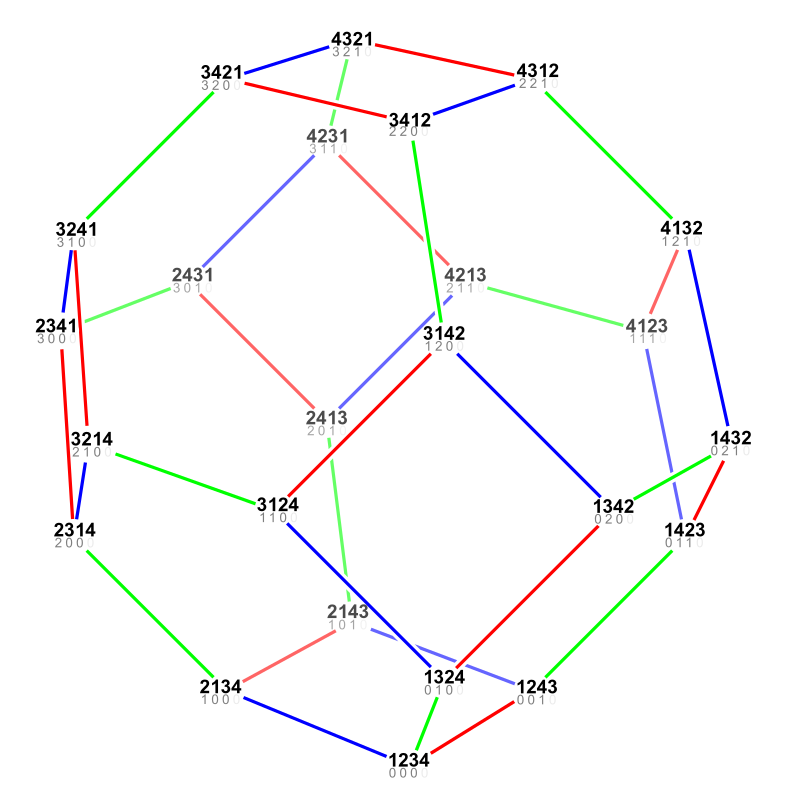
\includegraphics[scale=0.4]{permutohedron4.png}
    \end{minipage}
    \begin{minipage}{0.40\textwidth}
        \centering
        $\sigma_1 = (2,4,3,1) \hspace{0.2cm} \sigma_2 = (2,3,1,4)$ \\ \vspace{0.3cm}
        \begin{bmatrix}
            0 & 0 & 0 & 1 \\ 
            1 & 0 & 0 & 0 \\ 
            \mathbf{0} & \mathbf{0} & \mathbf{1} & \mathbf{0} \\ 
            0 & 1 & 0 & 0
        \end{bmatrix} 
        \stackrel{\text{(?)}}{\longrightarrow} 
        \begin{bmatrix}
            \mathbf{0} & \mathbf{0} & \mathbf{1} & \mathbf{0} \\ 
            1 & 0 & 0 & 0 \\ 
            0 & 1 & 0 & 0 \\ 
            0 & 0 & 0 & 1
        \end{bmatrix}$ \vspace{0.6cm} 
        \hspace{0.5cm}
        
        $\begin{bmatrix}
            0 & 0 & 0 & 1 \\ 
            1 & 0 & 0 & 0 \\ 
            0 & 0 & 1 & 0 \\ 
            0 & 1 & 0 & 0 
        \end{bmatrix} \stackrel{\text{(2 3)}}{\longrightarrow} 
        \begin{bmatrix}
            0 & 0 & 0 & 1 \\ 
            0 & 0 & 1 & 0 \\
            1 & 0 & 0 & 0 \\ 
            0 & 1 & 0 & 0
        \end{bmatrix} 
        \stackrel{\text{(1 2)}}{\longrightarrow} \\
        \vspace{0.2cm}
        \begin{bmatrix}
            0 & 0 & 1 & 0 \\
            0 & 0 & 0 & 1  \\ 
            1 & 0 & 0 & 0 \\ 
            0 & 1 & 0 & 0
        \end{bmatrix}$
        \stackrel{\text{(2 3)}}{\longrightarrow} \begin{bmatrix}
        0 & 0 & 1 & 0 \\ 
        1 & 0 & 0 & 0 \\
        0 & 0 & 0 & 1 \\
        0 & 1 & 0 & 0
        \end{bmatrix}$  $\stackrel{\text{(3 4)}}{\longrightarrow} \\
        \vspace{0.2cm}
        \begin{bmatrix}
       0 & 0 & 1 & 0 \\ 1 & 0 & 0 & 0 \\ 0 & 1 & 0 & 0 \\ 0 & 0 & 0 & 1
    \end{bmatrix}
    \end{minipage}
\end{posterbox}




\begin{posterbox}[name=refs, column=2,above=bottom]{References}
\bibitem{Convexity}
    Alexander Barvinok. \emph{A Course in Convexity} 
    \bibitem{Permuoahedron MIMUW}
    G. Lancia, P. Serafini. \emph{Compact Extended Linear Programming Models}
    
    \bibitem{Permutohedron v2}
    Micheal X. Goemans. \emph{Smallest Compact Forumlation for the Permutahedron}
\end{posterbox}

\begin{posterbox}[name=permutation3, column=0, below=Schur]{Permutohedron of (1,2,3) }
\includegraphics[scale=0.25]{permutohedron-3.png}
\end{posterbox}

\begin{posterbox}[name=eqdef,column=2,row=0]{Equivalent definition }
Let $[n] = \{1,...,n\}$ be a set of $n$ first natural numbers.
Set of points $x \in \mathbb{R}^n$ fulfilling $2^n - 2$ inequalities and one equality:

$$ \sum_{i \in J} x_i \geq \frac{|J|(|J|+1)}{2}, J \subset [n], J \neq \emptyset, J \neq  [n] $$

$$ \sum_{i=1}^{n} x_i = \frac{n(n+1)}{2} $$
is a Permutohedron.
\end{posterbox}
\begin{posterbox}[name=edges,column=2,row=1,below=eqdef]{Edges in Permutohedron}
There exists edge between
two vertices associated with two permutations $\sigma_1, \sigma_2$ if and only if there exists a transposition of two next elements  $\sigma_3 = (i $ $ i+1)$, $i=1,..n-1$ such that  $ \sigma_2 = \sigma_3 \circ \sigma_1$.
\newline 
It can be intuitively understood by the fact, that these are the closest neighbours in the standard Euclidian metric. 
\end{posterbox}

\begin{posterbox}[name=quest,column=2,below=edges]{Question}
    Since we can look at  $n$-dimensional Permutohedron as graph, interesting question is, how to find the shortest path between two vertices. 
\end{posterbox}
\begin{posterbox}[name=algorithm, column =1, span =2, below = permutation4]{Algorithm}
\begin{minipage}{0.30\textwidth}
     $\sigma_1 = (2,4,3,1)$  \newline \vfill
     $\begin{bmatrix}
        \mathbf{4: } \\ \mathbf{2: } \\ \mathbf{1: } \\ \mathbf{3: }  
    \end{bmatrix} \begin{bmatrix}
        0 & 0 & 0 & 1 \\ 1 & 0 & 0 & 0 \\ 0 & 0 & 1 & 0 \\ 0 & 1 & 0 & 0
    \end{bmatrix}$ \vfill
\end{minipage}
\begin{minipage}{0.30\textwidth}
    $\sigma_2 = (2,3,1,4)$  \newline \vfill
    $\begin{bmatrix}
        \mathbf{1: } \\ \mathbf{2: } \\ \mathbf{3: } \\ \mathbf{4: }  
    \end{bmatrix} \begin{bmatrix}
          0 & 0 & 1 & 0 \\ 1 & 0 & 0 & 0 \\ 0 & 1 & 0 & 0 \\ 0 & 0 & 0 & 1
    \end{bmatrix} $ 
\end{minipage}
\begin{minipage}{0.30\textwidth}
\vspace{0.35cm}
    Problem of finding the shortest path between two vertices is the same as problem of sorting an array swapping only adjacent elements.  \vspace{0.35cm}
\end{minipage}
    
\end{posterbox}
\begin{posterbox}[name=complexity,below=permutation3,column=0,span=2,above=bottom]{Complexity of Algorithm}
    An array to be sorted using only consecutive swaps, needs in edge case $\frac{n(n-1)}{2}$ iterations - which is also the diameter of Permutohedron, therefore shown algorithm is the fastest possible if our goal is to find the shortest path.
\newline 
If we only need a length of it, we can use approach similair to the merge sort algorithm, which can find an answer in $O(n\log(n))$ time
but the exact path cannot be found that way. 
\end{posterbox}
\end{poster}
\end{document}
